% -----------------------------------------------------------------------------------
\subsection{RMF Specification Editor}
% -----------------------------------------------------------------------------------

\begin{figure}
  \centering
  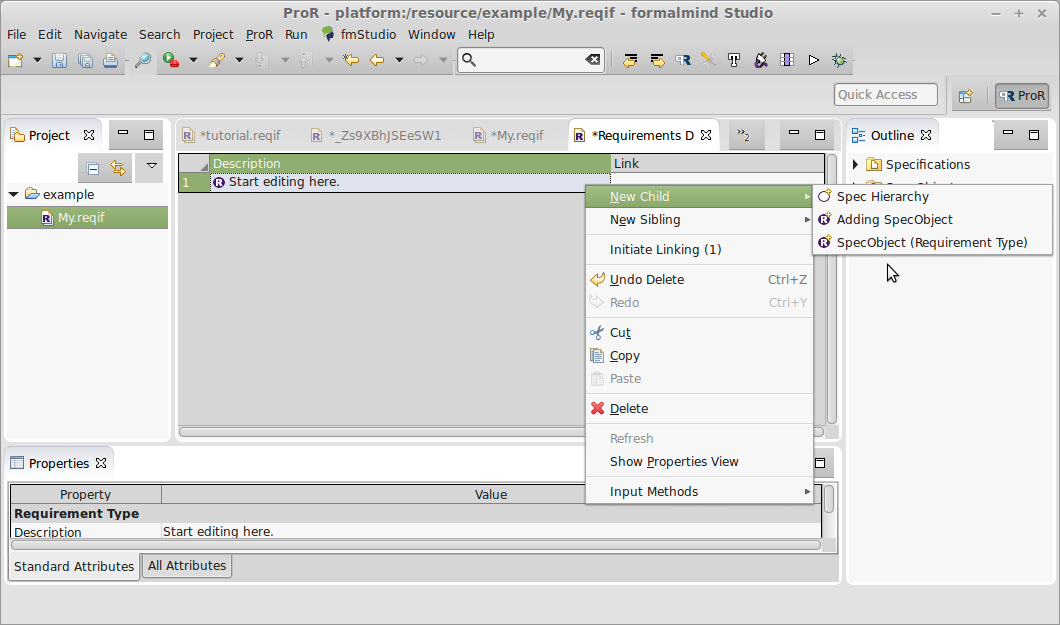
\includegraphics[width=\linewidth]{../rmf-images/default_spec_view.png}
  \caption{Specification Editor with the context menu open for creating a new child element}
  \label{fig:default specification editor}
\end{figure}

The Specification Editor shows the SpecObjects of a Specification, arranged in a grid view.  The hierarchy is shown via the indent of the first column, as well as through the numbering in the row header.

The columns show the Attributes with the names that match the column names (as shown in the header).  The columns can be resized by dragging.  Other operations, in particular reordering, adding and deleting columns are done via the \menu{Column Dialog}, accessible via \menu{Studio | Column Configuration } or the toolbar 
\includegraphics[height=0.8em]{../rmf-images/icons/full/obj16/Column.png}. 

The leftmost column shows the hierarchy and carries an icon.  The icon indicates whether it is a lone SpecHierarchy 
\includegraphics[height=0.8em]{../rmf-images/icons/full/obj16/spechierarchy.png} or a SpecObject 
\includegraphics[height=0.8em]{../rmf-images/icons/full/obj16/requirement.png}.

\begin{info}
Would you like to rearrange the columns?

In the top half of the \menu{Column Configurator} {
\includegraphics[scale=0.6]{../rmf-images/icons/full/obj16/Column.png}} window, a list of the exiting columns appear. Simply drag and drop them into the desired order. The changes appear in real time in the \menu{Specification Editor}. Close the window and the changes will be accepted.
\end{info}

Information can be entered either directly into the cell by double-clicking it or via the \menu{Properties View}.  While the Specification Editor only allows the editing of those attributes for which a column exists, the \menu{Properties View} will always show all attributes.

\begin{figure}
  \centering
  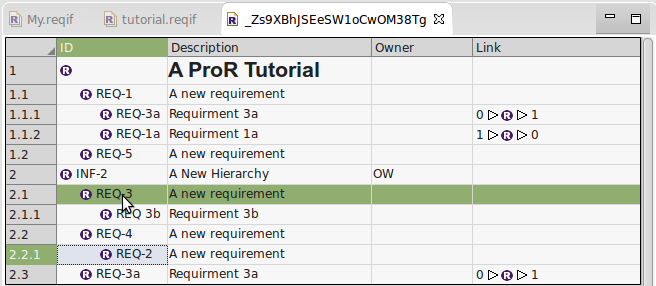
\includegraphics[width=0.8\linewidth]{../rmf-images/hierarchy_step_1.png}
  \caption{Click on a requirement and drag onto target parent.}
  \label{fig:hierarchy_step_1}
\end{figure}
\begin{figure}
  \centering
  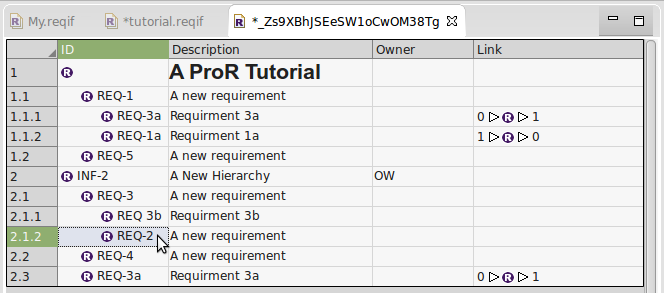
\includegraphics[width=0.8\linewidth]{../rmf-images/hierarchy_step_2.png}
  \caption{Result: The requirement is now a child of the chosen parent.}
  \label{fig:hierarchy_step_2}
\end{figure}

The SpecObjects can be reordered via drag and drop.  To move an existing SpecObject into the position of parent or child of another existing SpecObject, simply drag the child directly \textit{onto the target SpecObject}, as shown in Figure~\ref{fig:hierarchy_step_1}. The result is shown in Figure~\ref{fig:hierarchy_step_2}. 

Alternatively, as you drag the SpecObject \textit{onto the line below or above} the level you would like to move it to, it will become a sibling rather than a child of the SpecObject.  This is shown in Figure~\ref{fig:hierarchy_step_3}, with the resulting ordering shown in Figure~\ref{fig:hierarchy_step_4}.

\begin{figure}
  \centering
  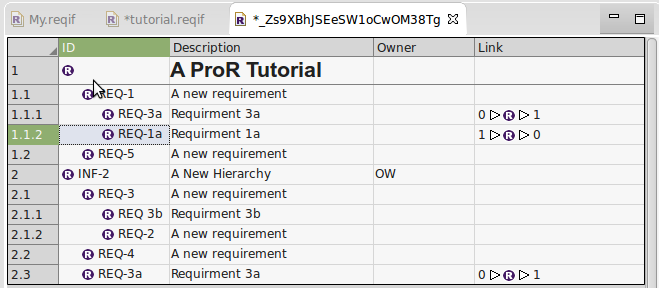
\includegraphics[width=0.8\linewidth]{../rmf-images/hierarchy_step_3.png}
  \caption{Click on a requirement and drag onto the line (bolded) below or above target sibling.}
  \label{fig:hierarchy_step_3}
\end{figure}
\begin{figure}
  \centering
  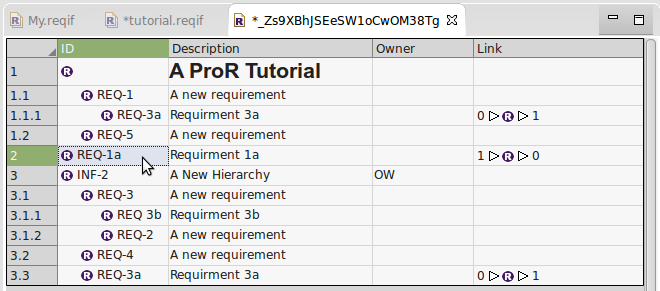
\includegraphics[width=0.8\linewidth]{../rmf-images/hierarchy_step_4.png}
  \caption{Result: The requirement is now a sibling of the chosen requirement.}
  \label{fig:hierarchy_step_4}
\end{figure}

To duplicate a SpecObject, simply copy and paste it into the required position. The copying, cutting and pasting functions are accessible through the traditional dropdown menu, by right-clicking on a desired cell or the corresponding keyboard shortcut.

By right clicking on any cell, you have a few options at your disposal. Outside of the usual \menu{Undo}, \menu{Cut}, \menu{Copy}, \menu{Paste} and \menu{Delete}, commands, the following are also available:

\begin{description}
\item
  [New Child.] A new SpecObject will be created as a child element.
\item
  [New Sibling.] A new SpecObject will be created as a sibling element.
\item
  [Initiate Linking.] This is the option to create a link between requirements. Once a link is initiated and then by right clicking a target selection, the options to complete the links either to or from a selection will appear. By default, the links are illustrated in the \menu{Link} column to the right. 
\item
  [Show Properties View.] Opens the \menu{Properties View}, where the selected element can be inspected and edited.
\end{description}

% -----------------------------------------------------------------------------------
\subsection{Project Explorer View}\index{project explorer}
% -----------------------------------------------------------------------------------

The \menu{Project Explorer View} is by default on the left side of the main window. Here you can inspect files and models associated with any project. If for some reason the Project Explorer View does not appear, Navigate to \menu{Window | Show View | Other | Project Explorer View}.

In the main area  of this viewer is a hierarchical listing of the project and it's components. Use the black arrow to the left to collapse or display the project's contents. Below the view's title and to the right are the options to collapse the project folder and link the project with the editor. To the right of these options is another dropdown menu.

This view is covered in more detail by the \eclipsehelp{/topic/org.eclipse.platform.doc.user/reference/ref-27.htm}{Eclipse documentation}.

% -----------------------------------------------------------------------------------
\subsection{ReqIF Validation}\index{validation}\index{ReqIF validation}
% -----------------------------------------------------------------------------------

ReqIF is spreading, and partners start handing .reqif and .reqifz files back and forth.  But chances are that the first import of such a file will fail.  What is the problem? Consequent, the free ReqIF-Validator may provide the answer.

The validation results are shown in the Eclipse Problem View.  In addition, it is possible to open the ReqIF file in question in a text editor and to generate error markers, as shown in Figure~\ref{fig:error-marker}.

\begin{info}
In addition to the validator that is built into the tool, there is also a command line version available, which can be downloaded for free from \url{https://reqif.academy}.
\end{info}

\begin{figure}
\centering     
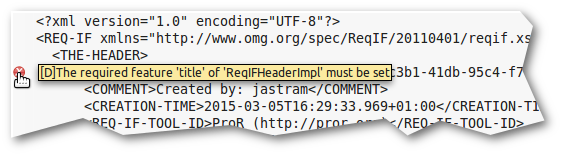
\includegraphics[width=\linewidth]{../rmf-images/error-marker.png}
\caption{Error Markers generated by Consequent}
\label{fig:error-marker}
\end{figure}

You can validate a ReqIF file as follows:

\begin{itemize}
\item    Right-Click the file to be validated in the Project Explorer (no need to open the file)
\item    Select \menu{Validate | Consequent ReqIF Validation}
\item    A dialog indicates the completion of the validation, which is shown in the Problem View.
\item    If the Problem View is not visible, open it by hand via \menu{Window | Show View | Other... | General | Problems}
\item    To see the error in the file, you must open it in a text editor as follows:
\begin{itemize}
\item        Right-Click the file in the Project Explorer
\item        Select Open With | Text Editor
\item        Errors are shown with an icon in the left margin (hovering over the error reveals the problem) – see screenshot below
\item        For errors with line numbers, it is possible to double click on an error in the Problem View to jump to the corresponding position in the Text Editor
\end{itemize}

\item    Error markers do not reset automatically. Re-run the validation to update them. You can manually clear error markes (e.g. for files that do not exist any more) by right-clicking on an element in the Problem View and selecting Delete.
\end{itemize}

\subsubsection{Validation Rules}

You can access and individually disable the validation rules via \menu{Window | Preferences | Model Validation | Constraints}.

\begin{info}
A printable version of the validation rules can retrieved from the build server at
\url{http://hudson.eclipse.org/rmf/job/rmf.develop.mars/ws/org.eclipse.rmf.reqif10.constraints/plugin.xml}
\end{info}

\subsubsection{Consequent Acknowledgement}

Consequent is part of the open source Eclipse project and was financed by the ProStep ReqIF Implementor Forum.

% ===================================================================================
\section{Configuration and Preferences}
% ===================================================================================

Both the current model, as well as \pror{} as a whole, can be configured and customized extensively.

% -----------------------------------------------------------------------------------
\subsection{Global Preferences}
\index{preferences}
% -----------------------------------------------------------------------------------

The application-wide settings of \pror{} are accessed via \menu{Window | Preferences | ReqIF}.  Configuration elements are:

\begin{description}
\item[ReqIF.] In the top level menu, the warning message for encountering simplified XHTML can be disabled.
\item[Default Presentations.] \pror{} has basic cell editors for each ReqIF \term{Datatypes}.  But it is possible to install new editors with better or different capabilities.  With this setting, Presentations can be selected to handle certain Datatypes by default.
\end{description}

\begin{info}
\index{XHTML}
Particularly popular is the free Presentation from Essentials for handling XHTML.  The standard editor from RMF converts rich text to plain text.  The rich text Presentation is preinstalled with ReqIF Studio.
\end{info}

% -----------------------------------------------------------------------------------
\subsection{General Configuration}
\index{configuration!general}
\label{sec:general_configuration}
% -----------------------------------------------------------------------------------

This configuration is accessed either via \menu{Studio | General Configuration}, or
via the 
\includegraphics[height=0.8em]{../rmf-images/ReqIFUIToolExtension.png} button on the toolbar.

Currently, there is only one configuration element: \menu{Label Configuration}.

% -----------------------------------------------------------------------------------
\subsubsection{Label Configuration}
\index{label configuration}
\index{configuration!label}
% -----------------------------------------------------------------------------------

The \menu{Label Configuration} is used to determine what to use for the text labels of elements
in places, where a shorthand is needed.  Examples are elements in the \menu{Outline View} or the link targets in the \menu{Link} column.

\pror{} will determine the label by looking at the label configuration, which is a list of Strings.
It will go through the list, top to bottom.  If the element has an attribute with a matching name,
that attribute value is used as the label.

If none is found, then the element's internal ID is displayed.

To configure, select \menu{Label Configuration} in the top pane of the dialog.  On the bottom pane, you see the \menu{Default Label} property.  Doubleclick the value (on the right), then click on the ellipses (...) to open the configuration dialog.  Under \menu{Feature}, you will see the list of attribute names that will be used for the label, if found.

Use the \menu{Add} and \menu{Remove} buttons to add more attribute names to be searched for.  The
search order can be adjusted with \menu{Up} and \menu{Down}.

\begin{info}
It is good practice to use the ID Presentation (\ref{sec:id_presentation}) to generate
user-friendly IDs, and to use these as the first match for a label.  As IDs are unique, you'll always
have a unique identifier that is typically also used for communication.
\end{info}

% -----------------------------------------------------------------------------------
\subsection{Datatype Configuration}
\index{configuration!datatype}
\index{datatype configuration}
\label{sec:datatype_configuration}
% -----------------------------------------------------------------------------------

\begin{figure}
\centering     
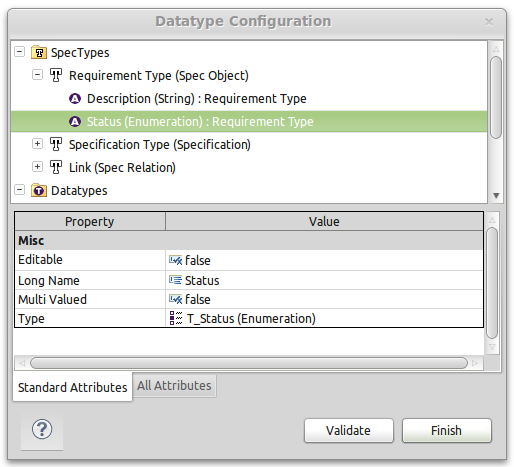
\includegraphics[width=0.8\linewidth]{../rmf-images/pror_datatype_configuration.png}
\caption{Datatype Configuration Dialog}      
\label{fig:DatatypeConfig}
\end{figure}

This configuration is opened via \menu{Studio | Datatype Configuration...}

The dialog shows two folders, one for SpecTypes and one for Datatypes.
SpecTypes are created for typing elements that have attributes
(SpecObjects, Specifications, SpecRelations).  New SpecTypes can be
created by right-clicking on the folder and selecting \menu{New Child}.
Through the same mechanism, attribute definitions can be added to a
SpecType.  Attribute definitions are typed.  Selecting an element shows
its properties in the lower pane, where it can be configured.

Attributes must have a name and a Datatype.  Some Attributes
allow further customization.  The Datatype is selected from a
dropdown.  New Datatypes can be created by right-clicking on the folder
\menu{Datatypes} and selecting \menu{New Child}.  Again, selecting a Datatype
shows its properties in the lower pane, where it can be configured.  A
Datatype should have at least the \menu{long name} property set.

As an example, consider the Datatype Configuration shown in Figure~\ref{fig:DatatypeConfig}.
The SpecType for ``Requirements Type,'' which is applicable to
SpecObjects, is expanded.  The SpecType has two Attributes,
``Description'' (String) and ``Status'' (Enumeration).  Status is
selected, and in the pane below the mandatory values, \menu{Long Name} and
\menu{Type} have been set.  Further customization of the attribute is
possible, e.g.  by converting it to a multi-valued Attribute by setting
the corresponding flag to \menu{true}.

\subsubsection{Enumeration Datatypes}

\begin{figure}
\centering      
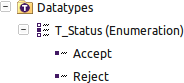
\includegraphics[width=0.3\linewidth]{../rmf-images/rmf_enumeration.png}
\caption{Enumerations}      
\label{fig:Enumerations}
\end{figure}

An Enumeration Datatype must have enumeration values.  These are created
by right-clicking the Enumeration Datatype and selecting \menu{New Child |Enum Value}.  You may have to unfold the enum value to select it, so that you can provide it with a \menu{Long Name}.  Figure~\ref{fig:Enumerations} shows a correctly configured Enumeration Datatype.

% -----------------------------------------------------------------------------------
\subsection{Presentation Configuration}\index{configuration!presentation}
\label{sec:presentation_configuration}
% -----------------------------------------------------------------------------------

Presentations are software components that extend the functionality of \pror{}.  Chapter~\ref{sec:presentations} is dedicated to Presentations.

% -----------------------------------------------------------------------------------
\subsection{Column Configuration}\index{configuration!column}
\label{sec:column_configuration}
% -----------------------------------------------------------------------------------

This configuration is specific to the Specification Editor.

The Column Configuration Dialog configures the Columns of a
Specification.  Columns are identified by name.  The width of the column
can be adjusted directly by dragging the column separator in the table
header.

If the SpecObject has an attribute where the name of the attribute
matches the name of the column, then that attribute is shown in that
column.

% ===================================================================================
\section{Access Control}
\index{access control}
\index{permissions}
\index{read-only}
% ===================================================================================

The ReqIF standard provides a flag for marking certain elements as read-only.  This flag is accessible through the \menu{Properties View} by selecting the tab \menu{All Attributes}.  However, this flag is not honored in the user interface: even if an element is marked as read-only, it is normally writable.  We may implement this in the future.

\begin{warning}
Access Control is a ReqIF feature designed for data exchange.  As \pror{} uses ReqIF as a data model (and not as an exchange format), access information is only stored, but not used for managing access.
\end{warning}

% ===================================================================================
\section{Import and Export}
% ===================================================================================

Importers and Exporters are accessed via \menu{File | Import...} and \menu{File | Export...}.  The corresponding dialogs will show generic Importers and Exporters, as well as specific ones.  The specific ones are in a folder called \menu{\pror{} (ReqIF)}.

This section also lists Importers and Exporters from third parties. Note that not all third-party Importers and Exporters may be listed here.

% -----------------------------------------------------------------------------------
\subsection{Import}
\index{import}
% -----------------------------------------------------------------------------------

The following importers exist:

\begin{description}
\item[ReqIFz Import.] This standard importer takes ReqIF archive (.reqifz) and imports it as an Eclipse project.

\item[CSV.] This standard importer takes comma-separated data and imports it into an existing ReqIF model.  It is described further below.

\item[Axiom.] This commercial importer supports the selective merging of exchange data with an existing ReqIF model.  It is described in detail in Section~\ref{sec:axiom}.

More information at the \href{https://reqif.academy}{ReqIF Academy}.

\end{description}

% -----------------------------------------------------------------------------------
\subsubsection{CSV Import}
\index{import!CSV}
% -----------------------------------------------------------------------------------

The CSV import adds the content from a comma-separated file into an existing specification.  Therefore, you first need to create a ReqIF model.  Once this is done, the importer is used as follows:

\begin{warning}
The importer will create new SpecTypes, Attributes and Datatypes.  Your existing types will not be reused!  We recommend to clean up the datatypes after the import.
\end{warning}

\begin{figure}
  \centering
  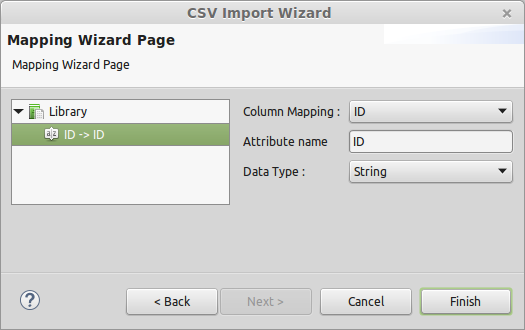
\includegraphics[width=0.8\textwidth]{../rmf-images/CSV_import.png}
  \caption{A complete mapping for a CSV import}
  \label{fig:csv}
\end{figure}

\begin{itemize}
\item Initiate the importer via \menu{File | Import... | ReqIF | CSV}.  

\item On the first dialog page, you need to select the source file containing the CSV data. The dialog defaults to comma-separated data, but other separators can be chosen as well.

\item A checkbox allows to indicated whether the file contains a header row.  If it is checked, the first row will be interpreted as the labels for the columns in the file.

\item Last, the destination model has to be chosen.  After this, the \menu{next} button is enabled.  

\item On the next page, the columns have to be mapped.  Initially, there is just a single element, \menu{Library}.

\item Right-click \menu{Library} to open the context menu that allows you to add a new mapping.  There are four options.  They all do the same, but the first three prepopulate the attribute name with a sensible value.

\item You need to create a mapping for each column that you would like to import.  A mapping consists of three elements:

\begin{description}
\item[Column Mapping.] Select the column from the CSV file.  The column headings are shown if the checkbox was selected on the previous page, otherwise just the column numbers.
\item[Attribute Name.] The name for the Attribute in the resulting ReqIF model.
\item[Data Type.] The datatype of the resulting attribute.  The safest option is \menu{String}, for other datatypes, a conversation attempt is made.
\end{description}

\item You do not need to create a mapping for all columns.  Figure\ref{fig:csv} shows the importer dialog with one complete mapping.

\item  Once all mappings are complete, hitting finish will complete the import.

\end{itemize}

You can read more in the \href{http://formalmind.com/blog/new-stuff-new-committer-new-product-new-importer-new-release}{Formal Mind Blog}.

% -----------------------------------------------------------------------------------
\subsection{Export}
\index{export}
% -----------------------------------------------------------------------------------

The following exporters exist:

\begin{description}
\item[ReqIFz Export.] This standard exporter takes an Eclipse project and produces a ReqIF archive (.reqifz).

\item[Axiom.] This commercial exporter supports the selective exporting of exchange data for supplier communication.  More information at the \href{https://reqif.academy}{ReqIF Academy}.

\item[HTML.] The HTML export is not a ``real'' export, as it is accessed differently.  It produces an HTML view from an open Specification.  To use it, you need to have a Specification Editor open.  Then select \menu{File | Print...}.
\end{description}

% ===================================================================================
\section{Searching and Filtering}
\label{sec:search}
\index{search}
% ===================================================================================

\pror{} has three search interfaces.  Each has a different focus:

\begin{description}
\item[Quicksearch (Section~\ref{sec:quicksearch}).] This interface allows search-as-you-type in the open editor.  It is useful for quickly finding the right row in a specification, but just performs a simple text search on all attributes.
\item[ReqIF Search (Section~\ref{sec:reqif_search}).] This interface allow the user-friendly construction of attribute-specific searches within the current model.
\item[Raw Search (Section~\ref{sec:raw_search}).] This interface is powerful, but requires the queries to be constructed by hand.  It allows to fine-tune the search scope, including the search of the whole workspace.
\end{description}

Except the quicksearch, the results are shown in the \eclipsehelp{/topic/org.eclipse.platform.doc.user/gettingStarted/qs-36b.htm}{Eclipse Search Result View}.

% -----------------------------------------------------------------------------------
\subsection{Quicksearch}
\label{sec:quicksearch}
\index{search!quicksearch}
\index{quicksearch}
% -----------------------------------------------------------------------------------

This feature allows you to search-as-you-type within the open Specification.  The search box is embedded in the toolbar and only visible if a Specification Editor is open.

\begin{center}

\includegraphics[height=3em]{../rmf-images/quicksearch.png}
\end{center}

You can just begin typing in the box.  With every keystroke, the view will update and collapse those rows that do not match.  All attributes are searched.

% -----------------------------------------------------------------------------------
\subsection{ReqIF Search}
% -----------------------------------------------------------------------------------

Searching is initiated via \menu{Search | Search... | ReqIF Search}, or via the search icon 
\includegraphics[height=1em]{../rmf-images/icons/full/obj16/search.png} on the toolbar.  This will present you the wizard shown in Figure~\ref{fig:reqif_search}.

\begin{info}
The search dialog shows several tabs on the top.  This handbook will cover ReqIF Search and ReqIF Search (Raw)---our ReqIF search tools.  

Depending on your Eclipse configuration, other search option may be shown and may still be useful.  For instance, the \eclipsehelp{/topic/org.eclipse.platform.doc.user/reference/ref-45.htm}{File Search} is useful for searching within all files, including .reqif files.
\end{info}

\begin{figure}
  \centering
  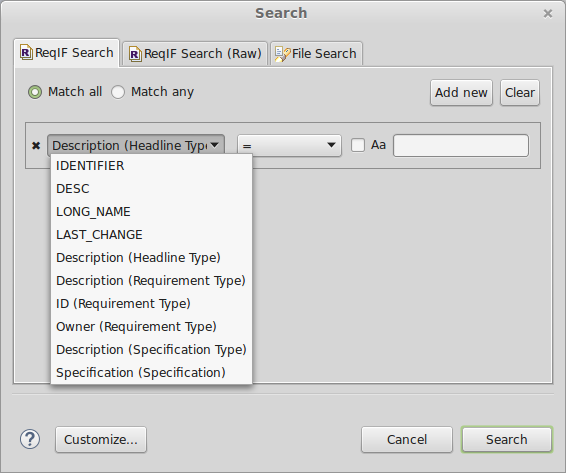
\includegraphics[width=0.8\textwidth]{../rmf-images/reqIF_search_1.png}
  \caption{ReqIF Search function with attribute dropdown menu}
  \label{fig:reqif_search}
\end{figure}
\label{sec:reqif_search}

% -----------------------------------------------------------------------------------
\subsubsection{Search Criteria}
% -----------------------------------------------------------------------------------

The ReqIF Search conditions consist of \textit{search criteria}, that are added by clicking on \menu{Add new}.  This creates a new criteria panel.  An arbitrary number of criteria can be defined.  Criteria can be removed by clicking on $\times$  on the left side of the panel, or by clicking \menu{clear} to remove all.

The radio button on top allows to either \menu{Match all} or \menu{match any} of the criteria.

Each criteria consists of three parts, \textit{attribute}, \textit{operator} and \textit{value}.  One such criteria is shown in Figure~\ref{fig:reqif_search}, with the attribute dropdown open.

\begin{description}
\item[Attribute.]  Choose an attribute (datatype) from the list.  The first four (IDENTIFIER, DESC, LONG\_NAME, and LA\-ST\-\_CHANGE) are ReqIF-internal attributes and are rarely of interest to normal users (see Section~\ref{sec:reqif_internal_attributes}).  The others attributes are taken directly from the document.  The more attributes you create, the longer the list will grow.  After you have chosen an attribute from the list, the rest of your choices (which are determined by the datatype of the attribute) are displayed.
\item[Operator.] The operator dropdown is specific to the selected attribute and is described for each type below.
\item[Value.] The value or values are specific to the operator and are also described below.
\end{description}

% -----------------------------------------------------------------------------------
\subsubsection{Operators for All Types}
% -----------------------------------------------------------------------------------

The following operators are available for all attributes, no matter what their type:

\begin{description}
\item[Equals (=).] For a match, the value must match \textit{exactly} as provided.  This implies that the attribute has actually been \textit{set}.  For instance, an empty string matches an empty string.  But it does not match if the value has not been set (i.e. if it is \textit{null}, in technical terms).
\item[Set.] For a match, the value must be set to any value. \textbf{Note:} A \term{default value} does not represent a match.
\item[Not set.] For a match, the value must not be set. \textbf{Note:} If the attribute in question does not exist, then there will not be a match either.  See example below.
\end{description}

\begin{example}
\textbf{Not Set Operator.}
Assume you receive a ReqIF model for review, with two SpecTypes, one called \textit{Information Type} which contains an attribute \textit{Description} and one called \textit{Requirement Type} which contains two attributes, \textit{Description} and \textit{Status}.  You are supposed to fill out the status for all requirements.

To find those that are still missing, you search for \menu{Status} \menu{not set}.  This will deliver all requirements for which no status has been set, even if there is a default value.
\end{example}

% -----------------------------------------------------------------------------------
\subsubsection{Operators for Plain and Rich Text}
% -----------------------------------------------------------------------------------

All text searches can be made case-sensitive by checking the corresponding checkbox \menu{Aa}.

The following operators are available for \textbf{plain text} attributes:

\begin{description}
\item[Not equals ($\neq$).] For a match, the value must not \textit{exactly} as provided.  If the attribute is not set, this constitutes a match.
\end{description}

The following operators are available for \textbf{plain text and rich text} (XHTML) attributes.

\begin{description}
\item[Contains.] For a match, the value must be a substring of the attribute.
\item[Contains not.] For a match, the value must not be a substring of the attribute. If the attribute is not set, this constitutes a match.
\item[Regexp.] The provided value will be interpreted as a \eclipsehelp{/topic/org.eclipse.platform.doc.isv/guide/st_text_types.htm?cp=2_0_3_9_1\#regex}{regular expression}.  Search will take place across line breaks.
\end{description}

\begin{info}
When searching rich text (XHTML), the invisible formatting will be included in the search, except for the \textit{regexp (plain)} operator described below.

Search will take place across line breaks.  But this is only relevant for Regexp search, where linebreaks can be matched explicitly (\menu{$\backslash$ n}) or as part of whitespace (\menu{$\backslash$ s}).
\end{info}

The following operators are available for \textbf{rich text} (XHTML) attributes.

\begin{description}
\item[Regexp (plain).] The provided value will be interpreted as a \eclipsehelp{/topic/org.eclipse.platform.doc.isv/guide/st_text_types.htm?cp=2_0_3_9_1\#regex}{regular expres\-sion}.  Search will take place against a version of the attribute value where the tags have been stripped out and been replaced by whitespace.
\end{description}

\begin{example}
\textbf{Searching XHTML.}  As XHTML contains invisible formatting tags, this should be taken into account when searching.  For instance, the search \menu{contains} \menu{formalmind.com} will find direct textual references to the domain, as well as hyperlinks. e.g. \texttt{<a href="http://for\-malmind.com">click</a>}.
\end{example}

% -----------------------------------------------------------------------------------
\subsubsection{Operators for Numbers (Integer and Real)}
% -----------------------------------------------------------------------------------

The interfaces for integer attributes and real attributes are identical, but the text boxes will only accept numbers of the appropriate type.

\begin{description}
\item[Not equal ($\neq$).] The provided value is not equal to the given number. This operator matches if the attribute has no value set.
\item[Between.] A match exists if the attribute value is between the given numbers, \textbf{including them}.
\item[Greater than ($>$).] A match exists if the attribute value is greater than the value, \textbf{excluding it}.
\item[Less than ($<$).] A match exists if the attribute value is less than the value, \textbf{excluding it}.
\end{description}

% -----------------------------------------------------------------------------------
\subsubsection{Operators for Dates}
% -----------------------------------------------------------------------------------

The granularity of the date criteria are one day, while \pror{} date stamps also include the time and have timezones.

\begin{warning}
\textbf{Timezones.} Dates in \pror{} have timezones.  The dates entered in the search interface assume the local time zone.  This can have implications if the values in the ReqIF model have been created by a user in a different time zone.  For example, consider a date has been written on ``Tuesday 23:00'' in the time zone of User~1.  But for User~2, it is already ``Wednesday 01:00''.  If User~1 would search for ``Tuesday'', there would be a match.  But for User~2, in a different time zone, not.
\end{warning}.

\begin{description}
\item[Equal ($=$).] The day matches, no matter what the time (but timezones apply).
\item[Not equal ($\neq$).] Any day except the given day, or not set.
\item[Between.] A match exists if the attribute value is between the given numbers, \textbf{including them}.
\item[Before.] A match exists if the attribute value is before the date, \textbf{excluding it} (i.e. before the time 00:00:00 on that date).
\item[After.] A match exists if the attribute value is after the date, \textbf{including it} (i.e. after the time 00:00:00 on that date).
\end{description}

% -----------------------------------------------------------------------------------
\subsubsection{Operators for Enumeration}
% -----------------------------------------------------------------------------------

While ReqIF enumerations may be single value or multi value, this distinction is immaterial for the search functionality.

\begin{description}
\item[Not equal ($\neq$).] Anything except an identical list will match.  \textbf{Note:} An empty list matches an unset attribute value.
\item[All.] All selected value must also be selected on the attribute (but the attribute may have more).
\item[Any.] For a match, at least one of the list values must also be set on the attribute.
\end{description}

% -----------------------------------------------------------------------------------
\subsubsection{Operators for Boolean}
% -----------------------------------------------------------------------------------

Only the standard operators (equals, set, not set) are available.

% -----------------------------------------------------------------------------------

% -----------------------------------------------------------------------------------
\subsection{Raw ReqIF Search}
\label{sec:raw_search}
\index{searcHraw ReqIF search}
\index{raw ReqIF search}
% -----------------------------------------------------------------------------------

The raw search feature has been described in the \href{http://formalmind.com/en/blog/formalmind-studio-pror-improvements-and-beta-program-about-start}{Formal Mind Blog}.

